\chapter{Alignment and Data Aquisition}

This chapter covers the steps for aligning a point-to-point focusing optic in
the beamline, and then collecting the data which will later be analyzed to
determine the optic's resolution and reflectivity with respect to energy. This
procedure is valid for bare nickel/nickel-cobalt optics as well as
multilayer-coated optics. A basic familiarity with the BLControl software is
assumed here, so please read Chapter~\ref{sec:software} first if you have not
done so already.

During the alignment process, there are a few things that you will need to
regularly check (every 15 minutes or so) and make note of in the log book:

\begin{itemize}

\item X-ray tube temperature: make sure it does not rise above $45^\circ$C
\item Detector temperature: should be below 230K for taking data
\item Radiation leakage: sweep the beamline periodically with the Geiger counter
  to check
\item Helium (if using) pressure and flow rate---see Section~\ref{sec:he} for
  details

\end{itemize}
In addition, while the x-ray source is on, you should always be wearing chest
and ring dosimetry.

\section{Setup and visual alignment}

Before starting the alignment, mount the detector and plug it in if
necessary. Make sure the detector and the motor controllers are connected to the
computer. Then, start up the software as described in
Section~\ref{sec:software}. During the initial alignment, leave the red cap or
blank tungsten pinhole on the end of the detector to protect the beryllium
window from damage.

Take note of the detector temperature and set point, displayed in the ``Detector
Control'' panel. If the detector has just been plugged in, it may need 10-15
minutes before it cools to below 220K, at which point it can be used.

The first step in the alignment process is to roughly align the optic and
detector by eye using visible light.

\begin{enumerate}

\item Start up the software. Make sure all motors appear in the ``Motor
  Control'' panel, and that the detector is cooling.

\item Remove all brass and copper pieces of shielding from the beamline and set
  them aside. Be careful not to bump any of the copper pipes into the detector.

\item Place the optic into the housing, and put the housing onto the v-block in
  the optic mount. If measuring in a magnifying configuration (i.e. the optic is
  closer to the source than to the detector), then the small end of the optic
  should point toward the sorce.

\item Using the optic $z$ stage (``\textit{oz}''), move the optic so that the
  inflection point is at the correct source-to-optic distance, as indicated in
  the optic design. Note that this distance is to the x-ray source spot, which
  is actually 1.22 inches behind the front flange of the x-ray
  tube\cite{tube_data_sheet}. Set this \textit{oz} location to zero in the
  software.

\item Move the detector $z$ stage to the center of its travel. By moving the
  stage assembly on the table, put the front window of the detector at the
  correct focal length as specified in the optic design, again keeping in mind
  that the x-ray source should be measured 1.22 inches behind the x-ray tube
  flange.

\item If the x-ray tube is currently mounted on the aluminum bracket, remove it
  and carefully set it aside. Attach the fiber optic holder to the aluminum
  bracket, with the copper collimator on the front. Insert the fiber optic
  output into the holder and turn on the white light source.

\item Replace the brass housing around the optic. If necessary, move the source
  or optic mounts so that the holes in the brass housing are centered with
  respect to the white light. Then, using the optic $x$ and $y$ stages
  (``\textit{ox}'' and ``\textit{oy}''), adjust the optic position so that it is
  centered with respect to the holes in the housing. Set these ``ox'' and ``oy''
  positions to zero in the software.

\item Holding a sheet of paper between the optic and the detector, locate the
  single-bounce focal spot. Adjust the pitch and yaw stages until the
  single-bounce focus appears symmetric. See Fig.~\ref{fig:vis_align} for
  reference images. Once pitch and yaw are aligned, set their positions to zero
  in the software.

\item Holding a sheet of paper in front of the detector, locate the
  double-bounce focal spot. Adjust the position of the detector in the $x$ and
  $y$ directions (``\textit{dx}'' and ``\textit{dy}'') until the focal spot
  coincides with the front window of the detector. Try to keep the \textit{dx}
  stage close to the center of its travel-- you may need to move the detector
  stage mount around on the table to achieve this.

\begin{figure}
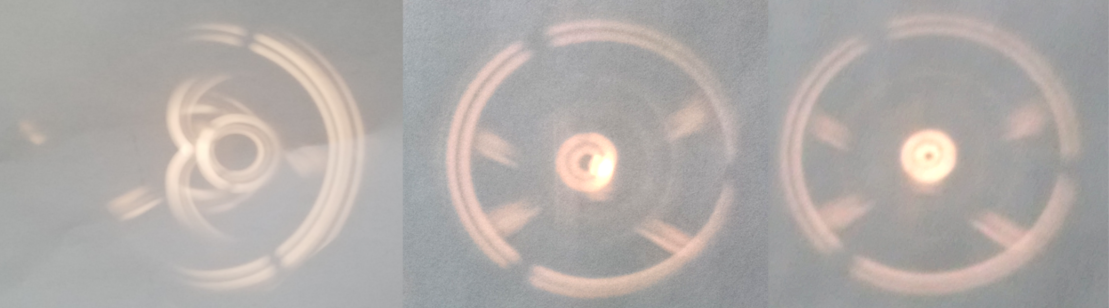
\includegraphics[width=\textwidth]{vis_align.png}
\caption{\label{fig:vis_align} Photos of the progression of the visible light
  alignment image. The leftmost image is highly asymmetric, indicating that the
  optic is still far off-axis, primarily in yaw. The center image is much closer
to proper alignment, but still slightly asymmetric, with the brightest portion
of the center spot skewed to the right. The rightmost photo shows a symmetric
alignment image, indicating a proper on-axis alignment.}
\end{figure}

\item Replace the copper pipes, starting with the pipe closest to the
  source. After placing each pipe, use a piece of paper at the end of the pipe
  to locate the beam of visible light, and adjust the position of the pipe so
  that the beam is centered. The pipes may not end up exactly parallel to the
  tabletop.

\item Remove the white light source and mount the x-ray tube. Take care not to
  move the source mount in the process, as doing so could alter the
  alignment. Use brass foil to cover any remaining gaps in the shielding. Remove
  the protective cap from the detector window.

\end{enumerate}


\section{Helium\label{sec:he}}

In this section, we will start the flow of helium through the copper shielding
pipes to reduce the attenuation of the x-rays (since helium has a much longer
attenuation length than air). This is only necessary if you want to measure low
energies (below about 5~keV), so for most multilayer-coated optics you can skip
to Section~\ref{sec:xrayalign}.

Note that if you are using helium, your count rate will probably be considerably
higher than what you are used to in air for a given tube current. You will
probably need to reduce the current accordingly so that the detector dead time
remains below 5\%.

\begin{enumerate}

\item Seal any connection points in the copper pipes to create a mostly airtight
  seal. Carefully wrapped duct tape many overlapping layers with few wrinkles)
  works fine for this.

\item Connect any tubing that runs from one pipe to another, so that helium can
  flow from one end of the beamline to the other.

\item Connect the helium tank to the tubing on one end of the beamline. You may
  want to use a needle valve between the tank and the copper pipe to give you
  greater control over the helium flow rate.

\item At the other end of the beamline, you should have one open section of
  tubing. Fill a beaker or other container with water and insert the open end
  into the water. When helium is flowing, it will bubble through the water and
  allow you to visualize the flow rate.

\item Open the helium tank. Using the tank regulator and the needle valve if
  present, adjust the output pressure until you see about one bubble every few
  seconds on the other end of the beamline. This should correspond to $<5$~psi
  of output pressure. If the pressure is too high, then stop the helium flow and
  check for leaks, especially at the points where two copper pipes come together
  (add more duct tape if using).

\item Once you have a decent flow rate at a sufficiently low pressure, you can
  move on to Section~\ref{sec:xrayalign}. While using helium, you need to keep
  an eye on the flow rate, output pressure, and amount of helium remaning in the
  tank. Check and record these values every 15~minutes or so while the helium is
  flowing, and adjust the output pressure if the flow rate becomes too high or
  if bubbles stop appearing.

\end{enumerate}

\section{Initial X-ray alignment\label{sec:xrayalign}}

In this section, we align the optic in pitch and yaw, and the detector in the
$x$ and $y$ directions (i.e. perpendicular to the optical axis).

\begin{enumerate}

\item Start up the x-ray source, as detailed in
  Section.~\ref{sec:src_startup}. The source voltage should be set so that the
  max energy is at least 5 keV above the energy range of interest (e.g. the
  location of the multilayer peak). All shielding should be in place at this
  time. Make sure to check periodically for radiation leaks and note the X-ray
  tube temperature.

\item Without setting an ROI, perform a $3\times3$ grid scan to find the center
  of the beam, and move \textit{dx} and \textit{dy} to this location.

\item If the optic has a multilayer, take a 30 second spectrum to find the
  multilayer peak. Set the ROI to encompass this peak. It should be wide enough
  to still encompass the entire peak, even if it shifts 1 or 2 keV in either
  direction during alignment, but should not encompass any ``stray peaks'' at
  lower energy.
%reword this^^

\textit{Note:} If the optic does not have a multilayer, then no ROI needs to be
set. From now on during the alignment process, if an ROI is set, then the ROI
peak or center of mass from a linear or grid scan should be used, as opposed to
the peak or center of mass of the total counts.

\item \label{itm:pit1} Perform a linear scan of \textit{pit}, $\pm 0.3 ^\circ$
  ($18$ arcminutes) in steps of $0.03^\circ$. 3-5 seconds of counting time per
  point should be sufficient. Move \textit{pit} to the center of the peak, and
  set it to zero.

\item \label{itm:yaw1} Repeat step~\ref{itm:pit1} for \textit{yaw}.

\item \label{itm:ox1} Scan \textit{ox} $\pm 1$~mm in steps of 0.2~mm. Move
  \textit{ox} to the center of the peak and set it to zero.

\item \label{itm:oy1} Repeat step~\ref{itm:ox1} for \textit{oy}.

\item Repeat steps \ref{itm:pit1} and \ref{itm:yaw1} for $\pm 0.2 ^\circ$ in
  steps of $0.02^\circ$, then repeat steps \ref{itm:ox1} and \ref{itm:oy1}.

\item \label{itm:all1} Repeat steps \ref{itm:pit1} and \ref{itm:yaw1} for $\pm
  0.1 ^\circ$ in steps of $0.01^\circ$, then repeat steps \ref{itm:ox1} and
  \ref{itm:oy1}.

\item \label{itm:pin3} Using a brass sheet to block the beam and shield your
  hand, place the 3~mm diameter pinhole on the end of the detector. Perform a
  $3\times3$ grid scan, with the step size the same as the pinhole diameter, and
  move to the center of mass.

\item \label{itm:all2} Scan and re-zero \textit{pit} and \textit{yaw} again $\pm
  0.1 ^\circ$ in steps of $0.01^\circ$, then scan and re-zero \textit{ox} and
  \textit{oy} $\pm 1$~mm in steps of 0.2~mm (as in step~\ref{itm:all1}).

\item Repeat steps \ref{itm:pin3} and \ref{itm:all2} with 2~mm and 1~mm diameter
  pinholes. Increase count time if necessary for better statistics. You may also
  reduce the size of the linear scans and use smaller steps to help refine the
  peak location, as long as the peak fits entirely within the bounds of the
  scan.

\textit{Note:} If the grid scan is still very symmetric with a 1~mm pinhole, you
can continue to step down to a 0.5~mm or even 0.25~mm pinhole. The smallest
pinhole that will be used depends on the resolution of the optic being measured,
but generally you should go as small as possible while the $3\times3$ grid scans
are still symmetric and have a well-defined beam center.

\item \label{itm:all3} With the smallest pinhole in place, continue to repeat
  the alignments of \textit{ox}, \textit{oy}, \textit{pit} and \textit{yaw}
  (linear scans) and \textit{dx} and \textit{dy} (grid scan). Repeat this cycle
  until the positions are no longer changing by more than $0.001^\circ$ or
  0.01~mm.

\end{enumerate}
This alignment may change slightly if the source is turned off, as the focal
spot within the tube can be in a different position each time it is powered
on. If the source is power cycled at any point, just repeat step~\ref{itm:all3}
to verify the alignment.

\section{Focus finding and HPD measurement\label{sec:focalign}}

Now that the optic is aligned with respect to the x-ray beam, and the detector
is aligned in the $xy$ plane, we will locate the focal point in the $z$
direction and calculate the resolution of the optic.

This section can be time-consuming, and you may want to skip it if you only care
about the optic's spectral response and don't need to know the resolution (or
already have good enough resolution data from a previous measurement). You are
likely to be close enough to the focal distance that the spectrum data will be
the same whether you find the exact focus or not. However, if you skip this
step, you will have to repeat the entire alignment process to get resolution
data in the future, so it's best to do it now if you think you might want it.

During this procedure, you are moving the detector back and forth along the beam
direction. Therefore, you must be careful to ensure that the detector does not
run into the copper shielding pipes. If you need to reposition the pipes to make
room for the detector to move, turn off the x-ray source first, and make sure
you don't hit the optic with the pipes while moving them.

\begin{enumerate}

\item Your current \textit{dz} position should be at the nominal focal length of
  the optic (measured manually during visual alignment) and should be set to
  $dz=0$. If not, set it to zero now.

\item \label{itm:smpin} With the smallest pinhole in place, re-center the
  detector using a grid scan. Then take a spectrum of about 30 seconds (you can
  alter this depending on your count rate) at the current position. Note in the
  log book how many counts are in your ROI.

\item \label{itm:nextpin} Change the pinhole to the next size up and repeat the
  spectrum for the same amount of time. Again note the ROI counts in the log
  book. Repeat this step with progressively larger pinholes, up to 5~mm
  diameter.

\item \label{itm:hpd} Following the instructions in Section~\ref{sec:hpd},
  calculate the HPD at the current position.

\item Move to $dz=20$~mm. Repeat steps \ref{itm:smpin}-\ref{itm:hpd}. If the HPD
  improves (i.e. decreases), continue another 20~mm in this direction. If it
  worsens, try the opposite direction. Continue moving in steps of 20~mm until a
  minimum in the HPD is found. Return \textit{dz} to the position where the HPD
  is minimized.

\textit{Note: }If you run out of travel on the \textit{dz} stage, you can return
\textit{dz} to the center of travel and move the entire stage assembly forward
or backward on the tabletop. Your position reference will be lost, so you will
need to re-center the detector in $x$ and $y$ and re-find the minimum HPD in
$z$.

\item \label{itm:10mm} Move \textit{dz} 10~mm in the direction of the next
  lowest HPD, and repeat steps \ref{itm:smpin}-\ref{itm:hpd}. If the HPD is
  lower, stay at this \textit{dz} position, otherwise return to the position of
  the minimum.

\item Repeat step~\ref{itm:10mm} for a move of 5~mm, and then for a move of
  2.5~mm.

\item Using the lowest measured value of the HPD, calculate the optic's spatial
  resolution as outlined in Section~\ref{sec:res}.

\end{enumerate}

\section{Spectrum data collection\label{sec:spec-collect}}

\begin{enumerate}

\item If you performed the focus finding alingment in
  Section~\ref{sec:focalign}, then move \textit{dz} to the location of the best
  measured HPD. Remove any pinhole from the detector and re-center by performing
  a $3\times3$ grid scan in 5~mm steps.

\item \label{itm:optspec} Collect a long spectrum (typically 10 minutes or more,
  depending on count rate) with no pinhole on the detector. When the acquisition
  is complete, make sure to save the spectrum file.

\item Turn off the x-ray source and remove the optic from the beamline. Place a
  3~mm pinhole on the detector. Re-start the source to the same current and
  voltage as before.

\item Collect a long spectrum without the optic for the same amount of time as
  in step~\ref{itm:optspec}. If, after one minute or so, the dead time of the
  detector is over 5\%, stop the acquisition, change the pinhole to a smaller
  diameter to reduce the count rate, and restart. Once the long spectrum is
  complete, make sure to save the spectrum file in the same directory as the
  file from step~\ref{itm:optspec}. Make sure to record which file is which
  (optic vs. no optic) and what size pinhole you used for the no optic spectrum.

\end{enumerate}

%%% Local Variables:
%%% mode: latex
%%% TeX-master: "Beamline_Manual"
%%% End:
